\chapter{Natural Deduction}
Mathematical proofs typically use a set of axioms along with some rules to derive a theorem. In this chapter we will look at a set of rules (called \indexit{Natural deduction}) to derive a theorem from a set of axioms. For a set of formulas $\Gamma$ and a formula $\beta$, we will denote by 
\[
\Gamma \proves \beta
\]
if using the rules in natural deduction and starting from the axioms $\Gamma$ we can derive the axiom $\beta$. There are two important properties the natural deduction set of rules satisfy.

\begin{theorem}[Soundness]
If $\Gamma \proves \beta$, then $\Gamma \models \beta$.
\end{theorem}

The soundness theorem shows that statements we can prove, are all true statements assuming the axioms are true. In other words, using the natural deduction proof rules, we cannot derive false theorems. Every proof system expects this property. A proof system without soundness does not make much sense. 
\begin{exercise}
Explain what the following statement mean? \\
If \true $~\proves \beta$, then \true $~\models \beta$.
\end{exercise} 

Natural deduction also satisfy the following interesting property. 
\begin{theorem}[Completness]
If $\Gamma \models \beta$, then $\Gamma \proves \beta$.
\end{theorem}
The completeness theorem says that, all true statements in the axiom system can be proved using the natural deduction proof rules. Mathematicians are interested in completeness. It assures them that all true theorems can be proved and therefore it is worthwhile to search for proofs. Do we have completeness for every logic? G\"odel showed that there is a logic which is not complete (infact the logic is embedded in set theory, making set theory not complete). That means there are true statements in the logic which cannot be proved.

If we want to say $\alpha \proves \beta$ and $\beta \proves \alpha$ then we use the notation $\alpha \dashv \proves \beta$. 

\section{Natural Deduction Rules}
We will now develop the rules to derive theorems from a set of axioms. Keep in mind that a proof is a sequence of formulas each of them generated by applying some rule on the previously generated formulas. Therefore, we need to identify rules by which we can introduce the logical symbols $\{\neg, \vee, \wedge, \ifthen\}$. We also need to identify rules by which each of these symbols can be eliminated along with proving some other formula. During the course of the lecture we will introduce and eliminate other symbols too.

\paragraph{And-introduction ($\andintro$)} Let us assume that we already have a proof of $\alpha$ and a proof of $\beta$. That is, starting from a set of axioms and applying the rules of natural deduction, we are able to prove $\alpha$ (and similarly $\beta$).
In other words, let us assume the following holds
\begin{align*}
\Gamma \proves \alpha \\
\Gamma \proves \beta 
\end{align*}
The and-introduction rule can now be applied to get a proof of $\alpha \wedge \beta$. That is,
\[
\Gamma \proves \alpha \wedge \beta 
\]

As you would expect the rule holds for any set of axioms. Hence we need a notation to represent the rules without mentioning the set of axioms. The following pictorial representation does this.

\begin{figure}[H]
\centering
\begin{prooftree}
\AxiomC{$\alpha$}
\AxiomC{$\beta$}
\RightLabel{\scriptsize $\andintro$}
\BinaryInfC{$\alpha \wedge \beta$}
\end{prooftree}
\caption{And-Introduction ($\andintro$)}
\end{figure}

On the top of the separating line we have $\alpha$ and $\beta$, the two formulas for which we already have a proof. The formula below the line is a consequent of the formulas mentioned above and applying the and-introduction rule. The rule is mentioned beside the line. This pictorial representation will be used for mentioning other rules.

\paragraph{And-elimination ($\andelim{1}$)} This rule, asks the following question. Let us assume we have a proof of $\alpha \wedge \beta$. What else can we infer from this? Isnt it true that if $\alpha$ and $\beta$ are true, both of them have to be true also. This is what the and-elimination rule says. If we can prove $\alpha \wedge \beta$, then we can prove $\alpha$ (and similarly $\beta$).

\begin{figure}[H]
\centering
\begin{subfigure}[b]{.1\linewidth}
\centering
\begin{prooftree}
\AxiomC{$\alpha \wedge \beta$}
\RightLabel{\scriptsize $\andelim{1}$}
\UnaryInfC{$\alpha$}
\end{prooftree}
\caption{$\andelim{1}$}
\end{subfigure}
~~~~~~~~~~~~~ \begin{subfigure}[b]{.1\linewidth}
\centering
\begin{prooftree}
\AxiomC{$\alpha \wedge \beta$}
\RightLabel{\scriptsize $\andelim{2}$}
\UnaryInfC{$\beta$}
\end{prooftree}
\caption{$\andelim{2}$}
\end{subfigure}
\caption{And-Elimination}
\end{figure}

The and-elimination has two rules. One to prove the left hand side of the conjunction. The other to derive the right hand side. Why do we require two rules? Isnt only the left rule enough? Note that the natural deduction rules does not assume any property of conjunction. In other words, it is not assumed that conjunction is a commutative operation. In fact commutativity is something we can prove using the rules we have seen till now.

Below we give the natural deduction for $(\alpha \wedge \beta) \wedge \gamma \vdash \alpha \wedge (\beta \wedge \gamma)$. We follow the notation used in Huth and Ryan.
\begin{figure}[H]
\centering
\begin{logicproof}{2}
  (\alpha \lor \beta)\lor \gamma & axiom \\
  \begin{subproof}
    (\alpha \lor \beta) & assumption\\
    \begin{subproof}
      \alpha & assumption\\
      \alpha\lor (\beta\lor \gamma) & $\orintro{1}$, 3
    \end{subproof}
    \begin{subproof}
      \beta & assumption\\
      \beta\lor \gamma & $\orintro{1}$, 5\\
      \alpha\lor (\beta\lor \gamma) & $\orintro{2}$, 6
    \end{subproof}
    \alpha\lor (\beta\lor \gamma) & $\orelim$, 2, 3--4, 5--7
  \end{subproof}
  \begin{subproof}
    \gamma & assumption\\
    \beta\lor \gamma & $\orintro{2}$, 9\\
    \alpha\lor (\beta\lor \gamma) & $\orintro{2}$, 10
  \end{subproof}
  \alpha\lor (\beta\lor \gamma) & $\orelim$, 1, 2--8, 9--11
\end{logicproof}
\caption{Proof}
\end{figure}

\begin{exercise}
Prove the following.
\begin{enumerate}
\item (commutative) $\alpha \wedge \beta \vdash \beta \wedge \alpha$.
\end{enumerate}
\end{exercise}

\paragraph{Double-negation elimination ($\doublenegelim$)} Consider the following statement
\myquote{``It is not true that it is not raining."}
The above statement uses two negations to say, ``It is raining". Our next rule says that such double negations can be eliminated.
\begin{figure}[H]
\centering
\begin{prooftree}
\AxiomC{$\neg\neg\alpha$}
\RightLabel{\scriptsize $\doublenegelim$}
\UnaryInfC{$\alpha$}
\end{prooftree}
\caption{Double negation-Elimination ($\doublenegelim$)}
\end{figure}

\paragraph{Double-negation introduction ($\doublenegintro$)} The double negation can be introduced by the following rule
\begin{figure}[H]
\centering
\begin{prooftree}
\AxiomC{$\alpha$}
\RightLabel{\scriptsize $\doublenegintro$}
\UnaryInfC{$\neg\neg\alpha$}
\end{prooftree}
\caption{Double negation-Introduction ($\doublenegintro$)}
\end{figure}


\paragraph{Implication-elimination ($\implelim$)} Implication elimination is something which is very natural. The high school mathematics has lots of proofs with implication elimination without explicitly mentioning it. This rule is also called as \indexit{modus ponens}. It says that, if we have a proof for $\alpha \ifthen \beta$ and we have a proof for $\alpha$, then $\beta$ can be derived. Note that, if formulas $\alpha \ifthen \beta$ is true and $\alpha$ is true, then $\beta$ is true necessarily (see truth table for implication). The rule for eliminating implication is given below
\begin{figure}[H]
\centering
\begin{prooftree}
\AxiomC{$\alpha$}
\AxiomC{$\alpha \ifthen \beta$}
\RightLabel{\scriptsize $\implelim$}
\BinaryInfC{$\beta$}
\end{prooftree}
\caption{Implication-elimination ($\implelim$)}
\end{figure}

\paragraph{Implication-introduction ($\implintro$)} This rule for introducing implication is a little tricky. It says that, if we assume $\alpha$ and are able to derive $\beta$, then we should be able to prove $\alpha \ifthen \beta$. It will require some time to convince yourself that this rule is not ``nonsense".  We denote this using our pictorial representation as follows.

\begin{figure}[H]
\centering
\begin{prooftree}
\alwaysNoLine
\AxiomC{$\alpha$}
\UnaryInfC{$.$}
\UnaryInfC{$.$}
\UnaryInfC{$.$}
\UnaryInfC{$\beta$}
\alwaysSingleLine
\RightLabel{\scriptsize $\implintro$}
\UnaryInfC{$\alpha \ifthen \beta$}
\end{prooftree}
\caption{Implication-introduction ($\implintro$)}
\end{figure}

\paragraph{Disjunction-introduction} Let us assume that we have a proof of $\alpha$. Then clearly we have a proof of $\alpha \vee \beta$, no matter what $\beta$ is. This is because if $\alpha$ is true, $\alpha \vee \beta$ is true for all $\beta$. The following rules introduces this disjunction symbol. Note that, since we do not know about the commutativity of disjunction we need two rules.

\begin{figure}[H]
\centering
\begin{subfigure}[b]{.1\linewidth}
\centering
\begin{prooftree}
\AxiomC{$\alpha$}
\RightLabel{\scriptsize $\orintro{1}$}
\UnaryInfC{$\alpha \vee \beta$}
\end{prooftree}
\caption{$\orintro{1}$}
\end{subfigure}
~~~~~~~~~~~~~ \begin{subfigure}[b]{.1\linewidth}
\centering
\begin{prooftree}
\AxiomC{$\beta$}
\RightLabel{\scriptsize $\orintro{2}$}
\UnaryInfC{$\alpha \vee \beta$}
\end{prooftree}
\caption{$\orintro{2}$}
\end{subfigure}
\caption{Disjunction-introduction}
\end{figure}

\paragraph{Disjunction-elimination ($\orelim$)} Let us assume we have a proof of $\alpha \vee \beta$. Moreover we have a proof of $\gamma$ assuming $\alpha$ as an axiom. Similarly we have a proof of $\gamma$ assuming $\beta$ as an axiom. We can therefore note that $\gamma$ should be provable from the original set of axioms. This is what disjunction elimination helps us achieve.

\begin{figure}[H]
\centering
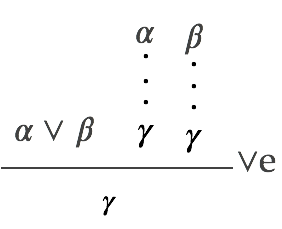
\includegraphics[scale=0.5]{orelim.png}
\caption{Disjunction-elimination ($\orelim$)}
\end{figure}

\begin{exercise}
Prove the following.
\begin{enumerate}
\item (commutative) $\alpha \vee \beta \proves \beta \vee \alpha$
\item (associative) $\alpha \vee (\beta \vee \gamma) \proves (\alpha \vee \beta) \vee \gamma$
\item (distributive) $\alpha \wedge (\beta \vee \gamma) \dashv \proves (\alpha \wedge \beta) \vee (\alpha \wedge \gamma)$.
\item $\alpha \vee (\beta \wedge \gamma) \dashv \proves (\alpha \vee \beta) \vee (\alpha \vee \gamma)$.
\end{enumerate}
\end{exercise}

\paragraph{False-elimination ($\falseelim$)} The rule says that, from a contradiction we can derive any formula. In other words, from falsity anything is provable. 
\begin{figure}[H]
\centering
\begin{prooftree}
\AxiomC{$\false$}
\RightLabel{\scriptsize $\falseelim$}
\UnaryInfC{$\alpha$}
\end{prooftree}
\caption{False-elimination ($\falseelim$)}
\end{figure}

\paragraph{Negation-elimination ($\negelim$)} Let us assume we are able to prove $\alpha$ and also prove $\neg \alpha$. Clearly we have proved a contradiction. The following rule can be used for proving contradictions.
\begin{figure}[H]
\centering
\begin{prooftree}
\AxiomC{$\alpha$}
\AxiomC{$\neg \alpha$}
\RightLabel{\scriptsize $\negelim$}
\BinaryInfC{$\false$}
\end{prooftree}
\caption{Negation-elimination ($\negelim$)}
\end{figure}

\paragraph{Negation-introduction ($\negintro$)} We are all used to proof by contradiction. This proof strategy assumes that a certain property is true and use that to prove a contradiction. This allow us to claim that our original assumption was wrong. This is exactly what this proof rule helps us to achieve.
\begin{figure}[H]
\centering
\begin{prooftree}
\alwaysNoLine
\AxiomC{$\alpha$}
\UnaryInfC{$.$}
\UnaryInfC{$.$}
\UnaryInfC{$.$}
\UnaryInfC{$\false$}
\alwaysSingleLine
\RightLabel{\scriptsize $\negintro$}
\UnaryInfC{$\neg \alpha$}
\end{prooftree}
\caption{Negation-introduction ($\negintro$)}
\end{figure}

Let us now some examples of natural deduction.

\begin{example}
Show that $\alpha \vee \beta, \alpha \vee \neg \beta \proves \alpha$.
\begin{figure}[H]
\centering
\begin{logicproof}{3}
  \alpha \vee \beta & axiom \\
  \alpha \vee \neg \beta & axiom \\
  \begin{subproof}
  \neg \alpha & assumption \\
  \begin{subproof}
	\begin{subproof}
		\alpha & assumption \\
  		\false & $\negelim$ 4,3 \\
  		\beta & $\falseelim$ 5
	\end{subproof}
	\begin{subproof}
  		\beta & assumption 
  	\end{subproof}
  		\beta & $\orelim$ 1, 4-6, 7
  	\end{subproof}
  	
  \begin{subproof}
   \begin{subproof}
		\alpha & assumption \\
  		\false & $\negelim$ 9,3 \\
  		\neg \beta & $\falseelim$ 10
  	\end{subproof}
	\begin{subproof}
  		\neg \beta & assumption 
  	\end{subproof}
  		\neg \beta & $\orelim$ 2, 9-11,12
  	\end{subproof}
  	\false & $\negelim$ 8,13
  	  	\end{subproof}
  	\neg \neg \alpha & $\negintro$ 3-14\\
  	\alpha & $\doublenegelim$ 15
\end{logicproof}
\caption{Proof of $\alpha \vee \beta, \alpha \vee \neg \beta \proves \alpha$}
\end{figure}
\end{example}

\begin{example}
Show that $\neg \alpha \proves \alpha \ifthen \beta$
\begin{figure}[H]
\centering
\begin{logicproof}{1}
	\neg \alpha & axiom \\
	\begin{subproof}
		\alpha & assumption \\
		\false & $\negelim$ 2, 1\\
		\beta & $\falseelim$ 3
	\end{subproof}
	\alpha \ifthen \beta & $\implintro$ 2-4
\end{logicproof}
\caption{Proof of $\neg \alpha \proves \alpha \ifthen \beta$}
\end{figure}
\label{example:negtoimpl}
\end{example}

\begin{example}
Show that $\neg \alpha \proves \neg (\alpha \wedge \beta)$
\begin{figure}[H]
\centering
\begin{logicproof}{1}
	\neg \alpha & axiom \\
	\begin{subproof}
		\alpha \wedge \beta & assumption \\
		\alpha & $\andelim{1}$ 2\\
		\false & $\negelim$ 3,1
	\end{subproof}
	\neg (\alpha \wedge \beta) & $\negintro$ 2-4
\end{logicproof}
\caption{Proof of  $\neg \alpha \proves \neg (\alpha \wedge \beta)$}
\end{figure}
\end{example}


\begin{exercise}[modus tollens] Show that $\alpha \ifthen \beta, \neg \beta \proves \neg \alpha$.
\label{exercise:modustollens}
\end{exercise}

\begin{exercise}[LEM]
Show that \true $~\proves \alpha \vee \neg \alpha$.
\label{exercise:lem}
\end{exercise}

\begin{figure}[H]
\centering
\includegraphics[width=1\textwidth]{allRules}
\caption{The rules of Natural Deduction}
\end{figure}


\section{Soundness theorem}
The proof of the theorem involves mathematical induction. If you are not used to induction, go through Chapter \ref{chap:mathInd}.

Let us restate the soundness theorem first.
\begin{theorem}[Soundness]
If $\Gamma \proves \psi$, then $\Gamma \models \psi$.
\label{thm:soundness}
\end{theorem}
The theorem says that, all formulas proved using natural deduction are true in a world where the axioms are true. The rest of this section will be devoted to proving the soundness theorem. The proof is by mathematical induction on the length of the proof. The length of a proof is the number of steps required in a natural deduction proof. The induction hypothesis is as follows:

\myquote{``For all set of formulas $\Gamma$, if $\Gamma \proves \psi$ where proof length is $n$, then $\Gamma \models \psi$ holds."}

Base Case ($n=1$): The only proof of length $1$ is as follows
\[
\Gamma \proves \alpha \text{~~--- Axiom}
\]
where $\alpha \in \Gamma$ is an axiom. From the definition of $\models$ it follows that $\Gamma \models \alpha$.

Inductive step: Let us assume that the induction hypothesis holds for all proofs of length less than or equal to $n$. We will show that the claim holds for proofs of length $n+1$. Consider one such proof. We will do a case analysis on the rule applied to derive $\psi$ in the $n+1$th step of the proof.

Case $\andintro$: The step is and-introduction. That is, we have $\Gamma \proves \psi$ and $\psi$ is of the form $\alpha \wedge \beta$ for some formulas $\alpha$ and $\beta$ which were derived earlier in the proof. Hence we know that $\Gamma \proves \alpha$ and $\Gamma \proves \beta$. From induction hypothesis (since the proof lengths are less than $n+1$) it follows $\Gamma \models \alpha$ and $\Gamma \models \beta$. From the semantics of $\wedge$, we get $\Gamma \models \alpha \wedge \beta$.

Case $\wedge e$: That means, $\Gamma \proves \psi$ and $\psi$ has been derived by applying an and elimination from a formula of the form $\psi \wedge \alpha$ or $\alpha \wedge \psi$. We will assume the former (the latter will have a symmetric argument). This means, there was a step in the proof which derived $\psi \wedge \alpha$ and hence $\Gamma \proves \psi \wedge \alpha$. Since the proof length of $\psi \wedge \alpha$ is less than $n+1$, from induction hypothesis we get $\Gamma \models \psi \wedge \alpha$. From the semantics of and ($\wedge$) it follows $\Gamma \models \psi$.

Case $\doublenegintro$: That is $\psi$ is of the form $\neg \neg \alpha$ for an $\alpha$ which was derived earlier in the proof. From induction hypothesis and semantics of negation (applied twice), it follows $\Gamma \models \psi$.

Case $\doublenegelim$: We can assume $\psi$ is got by elimination the double negation from a formula $\neg \neg \psi$ which was derived earlier in the proof. Again, applying induction hypothesis and using the semantics of negation, we get that $\Gamma \models \psi$.

Case $\implintro$: Let us assume that $\Gamma \proves \psi$ and $\psi$ is of the form $\alpha \ifthen \beta$ and the rule applied was implication-introduction. Therefore, after assuming $\alpha$, there is a derivation of $\beta$ in the proof. In other words, $\Gamma \cup \alpha \proves \beta$. This proof is of length less than $n+1$ and hence $\Gamma \cup \alpha \models \beta$. From the semantics of implication, it follows that $\Gamma \models \alpha \ifthen \beta$. 

Similarly going through all the other cases will finish the proof of the soundness theorem. The reader is asked to try showing this.

\begin{exercise}
Show the remaining cases, left out in Theorem \ref{thm:soundness}.
\end{exercise}

\section[Completeness: Huth \& Ryan]{Completeness theorem: Huth \& Ryan}
\label{sec:completeness}

We say that a formula $\alpha$ is a \indexit{theorem} if $\alpha$ can be proved without assuming any axioms. That is, $\true ~\proves \alpha$. 

In this section we prove the completeness theorem in a weaker setting, where $\Gamma$ is a finite set of formulas. The stronger result will be given later.
\begin{theorem}[Completeness]
\label{thm:completeness}
Let $\Gamma$ be a finite set of formulas. Then,  $\Gamma \models \psi$ implies $\Gamma \proves \psi$.
\end{theorem}
The theorem says that, if our formula is true in a world where the axioms are true, then the formula can be proved from the axioms. The rest of the section is proving the theorem. The proof strategy we follow is given in Figure \ref{fig:completenessHR}.

\begin{figure}[!h]
\centering
\begin{tikzpicture}[node distance = 0.75cm, auto]
    % Place nodes
    \node [block] (one) {1. Reduce completeness theorem to proving ``If $\alpha$ is a tautology then $\alpha$ is a theorem''.};
    \node [block, below of=one] (two) {2. For every valuation $v$, we give a formula $\beta_v$ and a proof  $\beta_v \proves \alpha$};
    \node [block, below of=two] (three) {3. We combine all the proofs above to show $\alpha$ is a theorem.};

    % Draw edges
    \path [line] (one) --node {} (two);
    \path [line] (two) --node {} (three);
    
\end{tikzpicture}
\caption{Proof of Completeness Theorem}
\label{fig:completenessHR}
\end{figure}

Our first step is to reduce the completeness theorem to a simpler case. 
\begin{lemma}
\label{lem:complete}
If $\alpha$ is a tautology, then $\alpha$ is a theorem. That is, if \true $~\models \alpha$, then \true $~\proves \alpha$
\end{lemma}

Before we prove the lemma, let us show how it would imply completeness theorem. Let us assume that $\Gamma = \{\alpha_1,\dots,\alpha_n\}$ and $\alpha_1,\alpha_2,\dots, \alpha_n \models \psi$.  From Exercise \ref{exercise:semequiv} we know this is equivalent to \true $~\models (\alpha_1 \wedge \alpha_2 \wedge \dots \alpha_n) \ifthen \psi$. Our Lemma \ref{lem:complete} shows that this is equivalent to \true $~\proves (\alpha_1 \wedge \alpha_2 \wedge \dots \alpha_n) \ifthen \psi$. From Exercise \ref{exercise:natequiv} it follows that $\alpha_1,\alpha_2,\dots,\alpha_n \proves \psi$. This finishes the completeness theorem.

Now we can go the proof of Lemma \ref{lem:complete}.
\begin{proof} [Proof of Lemma \ref{lem:complete}]
Let $P$ be the set of all propositions in $\alpha$. For a particular valuation, $v$ of $P$, we can define the following formula $\beta_v$ 
\[
\beta_v = \bigwedge_{\substack{p \in P \\ v(p) = \true}} p ~\wedge \bigwedge_{\substack{p \in P \\ v(p) = \false}} \neg p
\]
That is $\beta_v$ is the conjunction of all propositions which are assigned true in the valuation along with the neg of all propositions which are assigned false. Let $\alpha$ be an arbitrary formula. Then the following claim holds for any valuation $v$ because $\beta_v$ is satisfied by exactly one valuation, namely $v$. 
\begin{claim}
\[\beta_v \nmodels \alpha \mbox{ iff } \beta_v \models \neg \alpha\]
\end{claim}
See exercise \ref{exercise_uniqueval} for the proof of the above claim. We now prove the following for all subformulas $\psi$ of $\alpha$.
\begin{align}
\text{If } \beta_v \models \psi \text{ then } \beta_v \proves \psi \nonumber \\
\text{If } \beta_v \not \models \psi \text{ then } \beta_v \proves \neg \psi 
\label{align:induction}
\end{align}
The proof is by structural induction on the parse tree of $\alpha$. Let us do a case analysis of the type of node.

Case $\psi := p$: Let us first consider the case $\beta_v \models p$. Since $p$ is a conjunct in $\beta_v$ and-elimination gives us $\beta_v \proves p$. Now if $\beta_v \not \models p$, then $\beta_v \models \neg p$, which implies $\neg p$ is a conjunct in $\beta_v$. Therefore, $\beta_v \proves \neg p$.

Case $\psi := \gamma_1 \wedge \gamma_2$: Let us first consider the case $\beta_v \models \gamma_1 \wedge \gamma_2$. 
\begin{align*}
\text{Let } & \beta_v \models \gamma_1 \wedge \gamma_2 
\\ \implies & \beta_v \models \gamma_1 \text{ and } \beta_v \models \gamma_2  \tag{ semantics of and}
\\ \implies & \beta_v \proves \gamma_1 \text { and } \beta_v \proves \gamma_2  \tag{ induction hypothesis}
\\ \implies & \beta_v \proves \gamma_1 \wedge \gamma_2  \tag{ and-introduction}	
\end{align*}
Now let us prove the other if condition.
\begin{align*}
\text{Let } & \beta_v \nmodels (\gamma_1 \wedge \gamma_2) 
\\ \implies & \beta_v \models \neg (\gamma_1 \wedge \gamma_2) \tag{ definition of semantic entailment}
\\ \implies & \beta_v \models \neg \gamma_1 \vee \neg \gamma_2 \tag { Demorgan's law (proof in Exercise \ref{exercise:demorgansem})}
\\ \implies & \beta_v \nmodels  \gamma_1 \text{ or } \beta_v \nmodels  \gamma_2 \tag { semantics of or}
\\ \implies & \beta_v \proves \neg \gamma_1 \text { or } \beta_v \proves \neg \gamma_2 \tag { induction hypothesis}
\\ \implies & \beta_v \proves \neg \gamma_1 \vee \neg \gamma_2 \tag { or-introduction }
\\ \implies & \beta_v \proves \neg (\gamma_1 \wedge \gamma_2) \tag{ See Exercise \ref{exercise:demorgan} for this derivation}
\end{align*}

We have shown both sides of equation \ref{align:induction}. 

Case $\psi := \gamma_1 \vee \gamma_2$:  Let us first consider the case $\beta_v \models \gamma_1 \vee \gamma_2$. From the semantics of disjunction, it follows that $\beta_v \models \gamma_1$ or $\beta_v \models \gamma_2$. By induction hypothesis, we have $\beta_v \proves \gamma_1$ or $\beta_v \proves \gamma_2$. From or-introduction, it follows that $\beta_v \proves \gamma_1\vee\gamma_2$. Now let us assume $\beta_v \not \models \gamma_1 \vee \gamma_2$. From the semantics of disjunction and negation, it follows that $\beta_v \models \neg \gamma_1$ and $\beta_v  \models \neg \gamma_2$. By induction hypothesis, we have $\beta_v \proves \neg \gamma_1$ and $\beta_v  \proves \neg \gamma_2$. Now exercise \ref{exercise:demorgan} gives us $\beta_v \proves \neg (\gamma_1\vee \gamma_2)$.

Case $\psi := \neg \gamma$: Let us first assume $\beta_v \models \neg \gamma$. Therefore $\beta_v \nmodels \gamma$. From induction hypothesis, therefore it follows that $\beta_v \proves \neg \gamma$. Now, let us assume $\beta_v \nmodels \neg \gamma$. This is equivalent to $\beta_v \models \gamma$ which from induction hypothesis gives us $\beta_v \proves \gamma$. Introducing double negation will give us $\beta_v \models \neg \neg \gamma$.

Case $\psi := \gamma_1 \ifthen \gamma_2$: Let us consider the case $\beta_v \models \gamma_1 \ifthen \gamma_2$.
\begin{align*}
\text{Let } & \beta_v \models \gamma_1 \ifthen \gamma_2
\\ \implies & \beta_v \models \neg \gamma_1 \vee \gamma_2 \tag{ see Exercise \ref{exercise:implequiv}}
\\ \implies & \beta_v \nmodels \gamma_1 \text{ or } \beta_v \models \gamma_2  \tag{ semantics of or and negation}
\\ \implies & \beta_v \proves \neg \gamma_1 \text { or } \beta_v \proves \gamma_2  \tag{ induction hypothesis}
\\ \implies & \beta_v \proves \neg \gamma_1 \vee \gamma_2  \tag{ or-introduction}	
\\ \implies & \beta_v \proves \gamma_1 \ifthen \gamma_2 \tag{ see Exercise \ref{exercise:toimpl}}
\end{align*}

Now let us assume $\beta_v \not \models \gamma_1 \ifthen \gamma_2$. 
\begin{align*}
\text{Let } & \beta_v \nmodels \gamma_1 \ifthen \gamma_2
\\ \implies & \beta_v \models \neg (\neg \gamma_1 \vee \gamma_2) \tag{ see Exercise \ref{exercise:implequiv}}
\\ \implies & \beta_v \models \gamma_1 \text{ and } \beta_v \nmodels \gamma_2  \tag{ semantics of or and negation, demorgan}
\\ \implies & \beta_v \proves  \gamma_1 \text { and } \beta_v \proves \neg \gamma_2  \tag{ induction hypothesis}
\\ \implies & \beta_v \proves  \gamma_1 \wedge \neg \gamma_2  \tag{ and-introduction}	
\\ \implies & \beta_v \proves \neg (\gamma_1 \ifthen \gamma_2) \tag{ see Exercise \ref{exercise:toimpl}}
\end{align*}
Thus equation \ref{align:induction} is true for the implication case.

We have exhausted all the ways in which formulas can be built. Therefore, the claim in equation \ref{align:induction} holds. Let us go back to the lemma and assume its hypothesis,  $\true ~\models \alpha$. That is, for all valuations $v$ over the propositions, $\beta_v \models \alpha$. From our discussion above we have $\beta_v \proves \alpha$. Exercise \ref{exercise:theorem} now gives us $\true ~\proves \alpha$.
\end{proof}


\section[Completeness: Hintikka*]{Completeness: Alternate proof using Hintikka sets*}
In this section we give an alternate proof for completeness. We prove the simpler version, namely

\noindent {\bf Lemma \ref{lem:complete}.} \emph{If \true $~\models \alpha$, then \true $~\proves \alpha$}

As seen in the previous section, the above lemma along with the exercises \ref{exercise:semequiv} and \ref{exercise:natequiv}, will give us the completeness theorem. The rest of the section is for proving the above lemma.

Natural deduction gives us rules to derive proofs of statements. What is an important property these rules should satisfy? It should not help us to derive both a property and its negation. That is, we do not want natural deduction to satisfy $\true \proves \alpha$ and $\true \proves \neg \alpha$ for any formula $\alpha$. In fact if it does, then using natural deduction you can prove any formula. 
\begin{exercise}
If $\true \proves \alpha$ and $\true \proves \neg \alpha$, then $\true \proves \beta$ for all $\beta$.
\end{exercise}
So what we are interested in is a property called \indexit{consistency}. We say that a formula $\alpha$ is \indexit{consistent} if $\true ~\nproves \neg \alpha$. That is, $\alpha$ is consistent if there is no proof for $\neg \alpha$. Note that, this does not say that there is a proof for $\alpha$. The following theorem connects consistent formulas and Lemma \ref{lem:complete}. In fact, it also shows that natural deduction is consistent.
\begin{claim}
The following statements are equivalent.
\begin{enumerate}
\item If \true $~\models \alpha$, then \true $~\proves \alpha$
\item If $\neg \alpha$ is consistent, then $\neg \alpha$ is satisfiable.
\end{enumerate}
\end{claim}
\begin{proof}
$(1 \implies 2):$ Let $\neg \alpha$ be consistent. That is  \true $~\nproves \neg \neg \alpha$.
Therefore \true $~\nproves \alpha$ (otherwise contradiction by double-negation introduction). From $(1)$ we get \true $~ \nmodels \alpha$ and hence $\neg \alpha$ is satisfiable.

\noindent $(2 \implies 1):$ Let \true $~\models \alpha$. Therefore $\neg \alpha$ is not satisfiable. From $(2)$ we get $\neg \alpha$ is not consistent. In other words \true $~\proves \neg \neg \alpha$. The claim now follows from double-negation elimination.
\end{proof}
We will now prove that ``If $\beta$ is consistent, then $\beta$ is satisfiable". For a finite set $X$ of formulas, we say $X$ is consistent if the formula $\bigwedge_{\alpha \in X} \alpha$ is consistent. Given a consistent set $X$, we can extend the sets in a meaningful way as follows. Let us order all propositional logic formulas into a sequence
 \[\alpha_0,\alpha_1,\dots\]
We define $X_0 = X$ and for all $i \geq 0$ we define $X_{i+1}$ as follows.
\[
X_{i+1} = \begin{cases}
X_i \text{, if } X_i \cup \alpha_i \text{ is not consistent } \\
X_i \cup \alpha_i \text{, otherwise}
\end{cases}
\]

We now define the maximal consistent extension of $X$, (denoted by $\hat X$) as $\bigcup_{i \geq 0} X_i$. This maximal consistent set satisfy some interesting properties.
\begin{lemma}
Let $\hat X$ be as defined above. Then
\begin{enumerate}
\item For all  $i \geq 0$, $\alpha_i \in \hat X$ iff $\neg \alpha_i \notin \hat X$. 
\item For all  $i,j \geq 0$, $\alpha_i \wedge \alpha_j \in \hat X$ iff $\alpha_i \in \hat X$ and $\alpha_j \in \hat X$.
\item For all  $i,j \geq 0$, $\alpha_i \vee \alpha_j \in \hat X$ iff $\alpha_i \in \hat X$ or $\alpha_j \in \hat X$.
\item For all  $i,j \geq 0$, $\alpha_i \ifthen \alpha_j \in \hat X$ iff $\alpha_i \notin \hat X$ or $\alpha_j \in \hat X$.
\end{enumerate}
\label{lem:mcs}
\end{lemma}
\begin{proof}
We will prove each of the above claims.
\begin{enumerate}
\item Let $\alpha_j = \neg \alpha_i$ and $k = max \{i,j\}$. We show that  $\alpha_i \in X_k$ iff $\alpha_j \notin X_k$. Let $\beta = \bigwedge_{i=0}^k \alpha_i$. Let us first assume that both $\alpha_i$ and $\neg \alpha_i$ are not in $X_k$. Then, $\beta \wedge \alpha_i$ and $\beta \wedge \neg \alpha_i$ are not consistent. Therefore \true $~\proves \neg (\beta \wedge \alpha_i)$ and \true $~\proves \neg (\beta \wedge \neg \alpha_i)$. From Example \ref{example:negtoimpl}, it follows that \true $~\proves \neg \beta$. This is a contradiction, since $\beta$ is consistent. Now, let us assume both $\alpha_i$ and $\neg \alpha_i$ both are in $X_k$. That is, \true $~ \nproves \neg (\beta \wedge \alpha_i \wedge \neg \alpha_i)$. This is a contradiction from exercise \ref{exercise:lem}. Therefore either one of $\alpha_i$ or $\alpha_j$ should be in $X_k$ and hence in $\hat X$.
\item Let $\alpha_l = \alpha_i \wedge \alpha_j$ and $k = max\{i,j,l\}$. We show that  $\alpha_l \in X_k$ iff $\alpha_i \in X_k$ and $\alpha_j \in X_k$. Let $\beta = \bigwedge_{i=0}^k \alpha_i$. First, let us assume $\alpha_l \notin X_k$. That is, \true $~\proves \neg (\beta \wedge \alpha_i \wedge \alpha_j)$. From Demorgan's exercise \ref{exercise:demorgan} we know this is equivalent to \true $~\proves \neg \beta \vee \neg \alpha_i \vee  \neg \alpha_j$. Since $\beta$ is consistent, \true $~\nproves \neg \beta$. Therefore (semantics of disjunction) gives, \true $~\proves  \neg \alpha_i$ or \true $~\proves  \neg \alpha_j$. This shows that either $\alpha_i \notin X_k$ or $\alpha_j \notin X_k$. Now let us consider the other direction of the claim. Let $\alpha_i \notin X_k$ or $\alpha_j \notin X_k$. In other words, \true $~\proves  \neg \alpha_i$ or \true $~\proves  \neg \alpha_j$. Applying or-introduction and demorgan's laws we get \true $~\proves \neg (\beta \wedge \alpha_i \wedge \alpha_j)$. Therefore $\alpha \in X_k$. This proves the forward direction of the claim.
\end{enumerate}

We leave the rest of the claims for the reader to prove.
\end{proof}

\begin{exercise}
Prove the remaining cases in Lemma \ref{lem:mcs}.
\end{exercise}

Our next lemma says that if a formula $\beta$ is in $\hat X$, then $\beta$ is satisfiable. 
\begin{lemma}
If $\beta \in \hat X$, then $\beta$ is satisfiable.
\label{lem:consistimplsat}
\end{lemma}
\begin{proof}
Let $V$ be a set which contains either propositions or its negations. We define $V$ as follows. If $p \in \hat X$, then $p \in V$. On the other hand, if $p \notin \hat X$, then $\neg p \in V$. It is easy to see that, there is a satisfying assignment which makes all formulas in $V$ true. We are done, if we show that $V \models \beta$. We prove the following induction hypothesis by structural induction on subformulas of $\beta$.
\[
\gamma \in \hat X \iff V \models \gamma
\]

Case $\gamma=p$, a proposition: If $p \in \hat X$, by definition $V \models \gamma$. On the other hand, if $p \notin \hat X$, we have by definition $V \models \neg p$ and therefore $V \nmodels p$.

Case $\gamma = \neg \psi$: If $\neg \psi \in \hat X$, then (by properties of $\hat X$, Lemma \ref{lem:mcs}) $\psi \notin \hat X$. By our induction hypothesis it follows $V \nmodels \psi$ and therefore (semantics of negation) $V \models \neg \psi$. Let us assume $\neg \psi \notin \hat X$. By Lemma \ref{lem:mcs}, $\psi \in \hat X$, which by IH gives us $V \models \psi$. Therefore $V \nmodels \neg \psi$.

Case $\gamma = \psi_1 \wedge \psi_2$: If $\psi_1 \wedge \psi_2 \in \hat X$, then (Lemma \ref{lem:mcs}) $\psi_1 \in \hat X$ and $\psi_2 \in \hat X$. By IH, $V \models \psi_1$ and $V \models \psi_2$ and therefore $V \models \psi_1 \wedge \psi_2$. Let us now assume $\psi_1 \wedge \psi_2 \notin \hat X$. Therefore (Lemma \ref{lem:mcs}) $\psi_1 \notin \hat X$ or $\psi_2 \notin \hat X$. From IH, we get $V \nmodels \psi_1$ or $V \nmodels \psi_2$. Therefore $V \models \neg \psi_1 \vee \neg \psi_2$. Which by demorgan's laws proves the case.

We leave the rest of the case as exercise.
\end{proof}
\begin{exercise}
Prove the remaining cases in Lemma \ref{lem:consistimplsat}.
\end{exercise}

We now have enough understanding to prove the completeness theorem. \\

\noindent {\bf Proof of Lemma \ref{lem:complete}.} Let $\neg \alpha$ be consistent. Extend the set $X = \{\neg \alpha\}$ to $\hat X$, the maximal consistent set. Lemma \ref{lem:consistimplsat}, gives that all formulas in $\hat X$ are satisfiable and therefore $\neg \alpha$ is satisfiable too. \qed

\section{Strong Completeness*}
In Section \ref{sec:completeness} we saw the completeness theorem for the case when $\Gamma$ is finite. In this section we will show that the completeness theorem is true even for the infinite case. Compactness theorem will help us in this regard.

\begin{theorem}[Strong completeness]
Let $\Gamma$ be a set of formulas and $\psi$ be a formula. Then $\Gamma \proves \psi$ if $\Gamma \models \psi$.
\end{theorem}
\begin{proof}
Let $\Gamma \models \psi$. Therefore $\Gamma \nmodels \neg \psi$. It follows that $\Gamma \cup \neg \psi$ is not satisfiable. The compactness theorem of propositional logic (Theorem \ref{thm:propCompactness}) gives us that there exists a finite subset $\Gamma' \subseteq \Gamma$ such that $\Gamma' \cup \neg \psi$ is not satisfiable. Therefore we have $\Gamma' \nmodels \neg \psi$. In other words $\Gamma' \models \psi$. From the completeness theorem for propositional logic (see Theorem \ref{thm:completeness}) we have $\Gamma' \proves \psi$. Since $\Gamma' \subseteq \Gamma$, we have $\Gamma \proves \psi$.
\end{proof}

\section{Exercises}
\begin{exercise}[syntactic variant of De Morgan's law]
Prove the following.
\begin{multicols}{2}
\begin{enumerate}
\item $\neg (\alpha \wedge \beta) \dashv \proves \neg \alpha \vee \neg \beta$
\item $ \neg \alpha \wedge \neg \beta \dashv \proves  \neg (\alpha \vee \beta)$
\end{enumerate}
\end{multicols}
\label{exercise:demorgan}
\end{exercise}

\begin{exercise}[Hilbert's axioms]
Prove the following.
\begin{multicols}{2}
\begin{enumerate}
\item \true $~ \vdash \big(\alpha \ifthen (\beta \ifthen \alpha)\big)$
\item \true $~ \vdash \big(\neg \beta \ifthen \neg \alpha \big) \ifthen \big(\alpha \ifthen \beta \big)$
\end{enumerate}
\end{multicols}
\begin{enumerate} 
\item [3.] \true $~ \vdash \big(\alpha \ifthen (\beta \ifthen \gamma)\big) \ifthen \big((\alpha \ifthen \beta) \ifthen (\alpha \ifthen \gamma)\big)$
\end{enumerate}
\end{exercise}

\begin{exercise}
Show that the following are equivalent
\begin{multicols}{2}
\begin{enumerate}
\item $\alpha_1, \alpha_2, \dots, \alpha_n \proves \beta$
\item \true $~\proves (\alpha_1 \wedge \alpha_2 \wedge \dots \alpha_n) \ifthen \beta$
\end{enumerate}
\end{multicols}
\begin{enumerate}
\item [3.] \true $~\proves \Big(\alpha_1 \ifthen \big(\alpha_2 \ifthen (\dots (\alpha_n \ifthen \beta))\big)\Big)$
\end{enumerate}
\label{exercise:natequiv}
\end{exercise}

\begin{exercise}
Prove the following.
\begin{multicols}{2}
\begin{enumerate}
\item $\neg \gamma_1 \vee \gamma_2  \dashv \proves \gamma_1 \ifthen \gamma_2$ 
\item $\gamma_1 \wedge \neg \gamma_2  \dashv \proves \neg (\gamma_1 \ifthen \gamma_2)$	 
\item $\neg \alpha \proves \alpha \ifthen \beta$
\item $\alpha \ifthen \beta, \beta \ifthen \alpha \proves \alpha \ifthen \gamma$
\end{enumerate}
\end{multicols}
\label{exercise:toimpl}
\end{exercise}

\begin{exercise}
Show that the following are theorems
\begin{multicols}{2}
\begin{enumerate}
\item $\alpha \vee \neg \alpha$
\item $\alpha \ifthen \alpha$
\item $\alpha \ifthen \neg \neg \alpha$
\item $(\alpha \ifthen \beta) \ifthen (\neg \beta \ifthen \neg \alpha)$
\item $(\neg \alpha \ifthen \alpha) \ifthen \alpha$
\item $ (\neg \alpha \ifthen (\alpha \ifthen \beta))$
\item $ \neg \neg \alpha \ifthen \alpha$
\item $(\alpha \ifthen \beta) \ifthen ((\alpha \ifthen \neg \beta) \ifthen \neg \beta))$
\end{enumerate}
\end{multicols}
\end{exercise}



\begin{exercise}
Let $\Psi$ be a formula over only the proposition $p$. Assume that $p \proves \psi$ and $\neg p \proves \psi$. Show that,  \true $~\proves \psi$.
\end{exercise}

\begin{exercise}
 Let us introduce a new connective xor: $\alpha \xor \beta$ which should abbreviate $(\neg \alpha \wedge \beta) \vee (\alpha \wedge \neg \beta)$. Design introduction and elimination rules for xor.
\end{exercise}

\begin{exercise}
Let $P = \{p_1,\dots,p_n\}$ be a set of propositions. For a valuation $v$ over $P$, we define $\Gamma_v = \{p_i ~|~ v(p_i) = \true \} \cup \{\neg p_i ~|~ v(p_i) = \false \}$. Consider a formula $\alpha$ such that $\Gamma_v \proves \alpha$ for all valuation $v$. Show that $\true ~\proves \alpha$.
\label{exercise:theorem}
\end{exercise}

\begin{exercise}
\label{exercise_uniqueval}
Let $v$ be a valuation. Then the following holds for all formulas $\alpha$.
\[
\beta_v \nmodels \alpha \mbox{ iff } \beta_v \models \neg \alpha
\]
\end{exercise}

\begin{exercise}
[Strong soundness theorem] If $\Gamma \proves \alpha$ then $\Gamma \models \alpha$.
\end{exercise}
\begin{exercise}
If $\Gamma$ is satisfiable then $\Gamma$ is consistent.
\end{exercise}

\begin{exercise}
Consider a new natural deduction set of rules you have created. Let $\Gamma$ be a set of propositional formulas (the set need not be finite). Let us also define by $\Gamma \proves^* \alpha$ to be a proof of $\alpha$ from $\Gamma$ using your natural deduction rules. Let us also say that $\Gamma$ is consistent, if you cannot prove $\alpha$ or $\neg \alpha$ using your natural deduction rules for any $\alpha$ from $\Gamma$. Prove that the following two statements are equivalent.
\begin{enumerate}
\item If $\Gamma \proves^* \alpha$ then $\Gamma \models \alpha$.
\item If $\Gamma$ is satisfiable then $\Gamma$ is consistent.
\end{enumerate}
\end{exercise}

\begin{exercise}
Design introduction and elimination rules for Nand operator. Consider the logic which uses only negation and Nand operator as logical symbols. Prove the completeness theorem using the introduction and elimination rules for Nand and negation. Prove also the soundness theorem.
\end{exercise}
 
\begin{exercise}
Prove the deduction theorem for a set (need not be finite) $\Gamma$ of propositional formulas : $\Gamma \proves (\alpha \ifthen \beta)$ iff $\Gamma \cup \{\alpha\} \proves \beta$.
\end{exercise}

\begin{exercise}
Prove or disprove the following statements.
\begin{enumerate}
\item If $\Gamma_1 \subseteq \Gamma_2$ and $\Gamma_1$ is consistent then $\Gamma_2$ is consistent.
\item If $\Gamma_1 \subseteq \Gamma_2$ and $\Gamma_2$ is consistent, then $\Gamma_1$ is consistent.
\end{enumerate}
\end{exercise}